\chapter{Contour Based Seed Point Location}
\lhead{\emph{Contour Based Seed Point Location}}

The ideal place to aim to flood fill a space from would be the centre point of the space. OpenCV provides the functionality to take the Canny output image (a matrix of colour values) and convert it into a set of contours. Contours are line objects stored in a hierarchical structure and have functions that can provide the centre point of each contour. Although the centre points of the contours will not map exactly to the centre points of the space, they are close enough approximations to flood fill from (Figure \ref{fig:ContourCentres}).

Unfortunately, due to a combination of the processing time required to convert the lines into contours and the number of contours produced that have no impact on the spaces left to be flood filled, this method is too resource heavy to produce 10 fps on a laptop, therefore is also too resource heavy for use on the raspberry pi.

\begin{figure}[H]
    \begin{center}
    \begin{tabular}{ c c }
        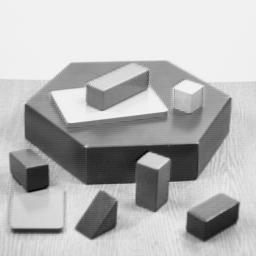
\includegraphics[width=0.31\textwidth]{Figures/blox.jpg} &
        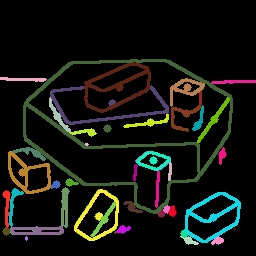
\includegraphics[width=0.31\textwidth]{Figures/ContourCentres.jpg}
    \end{tabular}
    \caption[Demonstration of contour centre point location]{Demonstration of contour centre point location. The original image (provided by OpenCV) on the left has been Canny edge detected, these edges have converted into contours, and the centre points of these contours located. The results of this are displayed on the right, with each contour and its corresponding centre point in a different colour. It can be observed that the centre points provide adequate coverage of the black spaces in the image to be used as seed points for flood filling.}
    \label{fig:ContourCentres}
    \end{center}
\end{figure}
